\let\negmedspace\undefined
\let\negthickspace\undefined
\documentclass[journal,12pt,twocolumn]{IEEEtran}
\usepackage{float}
\usepackage{circuitikz}
\usepackage{cite}
\usepackage{amsmath,amssymb,amsfonts,amsthm}
\usepackage{algorithmic}
\usepackage{graphicx}
\usepackage{textcomp}
\usepackage{xcolor}
\usepackage{txfonts}
\usepackage{listings}
\usepackage{amsmath}
\usepackage{enumitem}
\usepackage{mathtools}
\usepackage{gensymb}
\usepackage{comment}
\usepackage[breaklinks=true]{hyperref}
\usepackage{tkz-euclide} 
\usepackage{listings}
\usepackage{gvv}                                        
\def\inputGnumericTable{}                                 
\usepackage[latin1]{inputenc}                                
\usepackage{color}                                            
\usepackage{array}                                            
\usepackage{longtable}                                       
\usepackage{calc}                                             
\usepackage{multirow}                                         
\usepackage{hhline}                                           
\usepackage{ifthen}                                           
\usepackage{lscape}
\newtheorem{theorem}{Theorem}[section]
\newtheorem{problem}{Problem}
\newtheorem{proposition}{Proposition}[section]
\newtheorem{lemma}{Lemma}[section]
\newtheorem{corollary}[theorem]{Corollary}
\newtheorem{example}{Example}[section]
\newtheorem{definition}[problem]{Definition}
\newcommand{\BEQA}{\begin{eqnarray}}
\newcommand{\EEQA}{\end{eqnarray}}
\newcommand{\define}{\stackrel{\triangle}{=}}
\newcommand{\systemZ}[1]{\stackrel{#1}{\mathcal{Z}}}

\theoremstyle{remark}
\newtheorem{rem}{Remark}
\begin{document}

\bibliographystyle{IEEEtran}
\title{ AUDIO FILTERING ASSIGNMENT}
\author{EE23BTECH11011- Batchu Ishitha$^{*}$% <-this % stops a space
}
\maketitle

\bigskip

\renewcommand{\thefigure}{\theenumi}
\renewcommand{\thetable}{\theenumi}
%\renewcommand{\theequation}{\theenumi}

\section{DIGITAL FILTER}
\begin{enumerate}[label=\thesection\arabic*.,ref=\thesection.\theenumi]
\item The sound file used for this code can be obtained from the following link.
\begin{lstlisting}
https://github.com/BATCHUISHITHA/EE-1205/blob/main/audio_filtering/codes/ishitha.wav
\end{lstlisting}
\item Python code for removal of out of band noise:
\lstinputlisting{./codes/1.2.py}  \label{1.2}
\item Analysis of sound file before and after removal of noise using spectrogram ie: https://academo.org/demos/spectrum-analyzer.
\solution
The darker areas are those where the frequencies have very low intensities, and the orange and the yellow areas represent the frequencies that have high intensities in sound.
\begin{figure}[ht]
    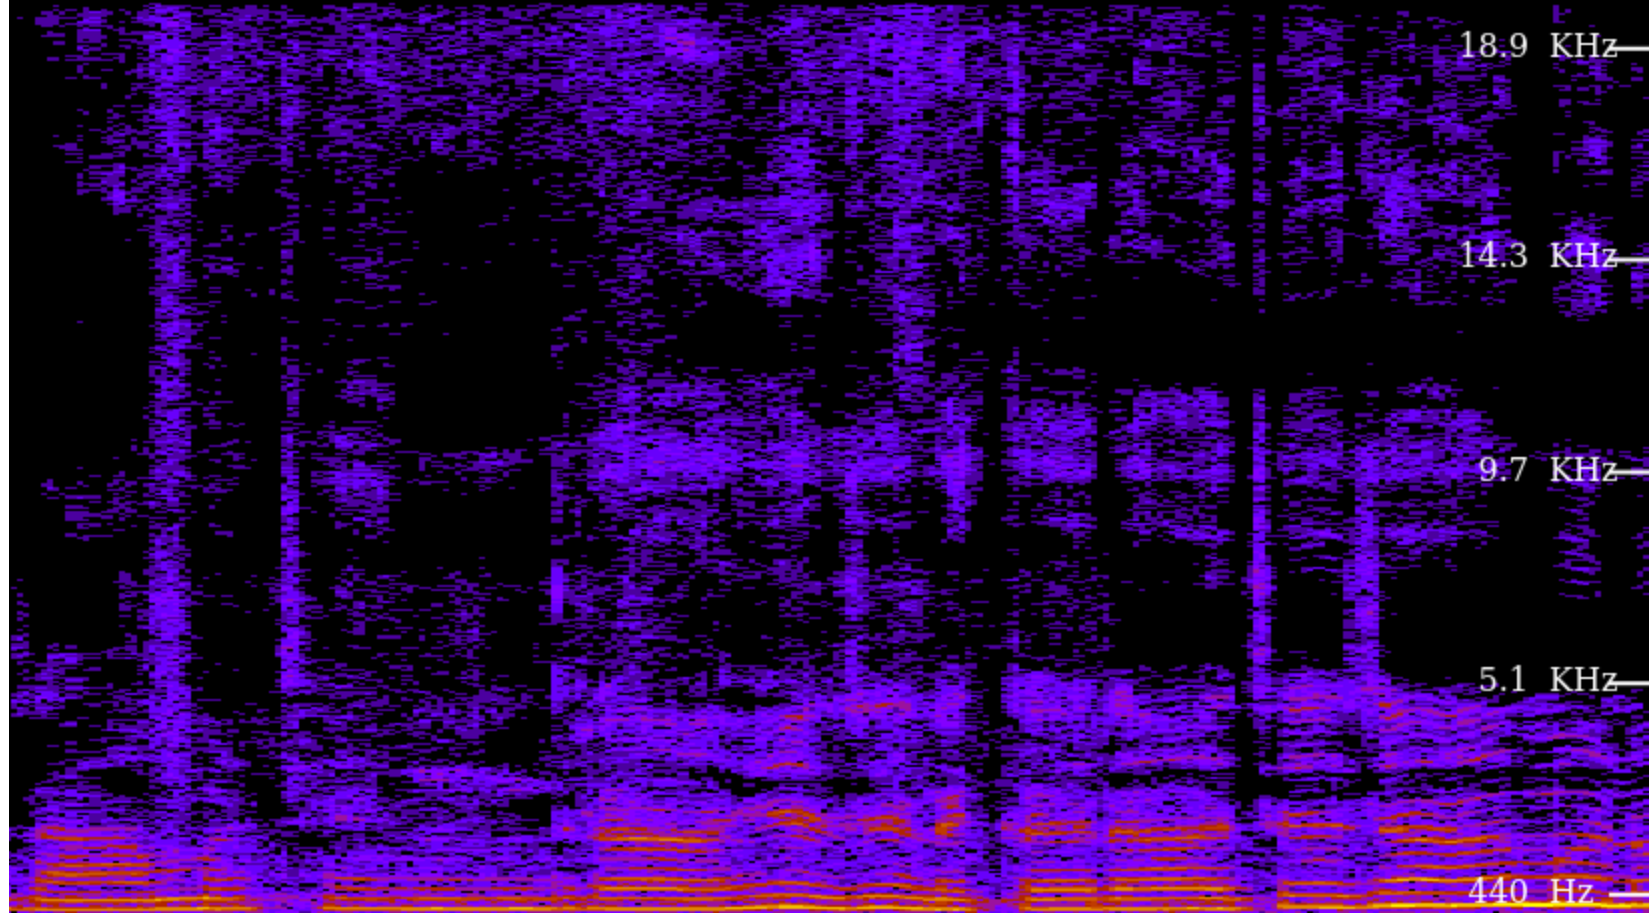
\includegraphics[width=0.8\columnwidth]{figs/beforefiltering.png }
    \caption{Spectrogram of the audio file before Filtering}
    \label{fig:beforefiltering}
\end{figure}
\begin{figure}[ht]
    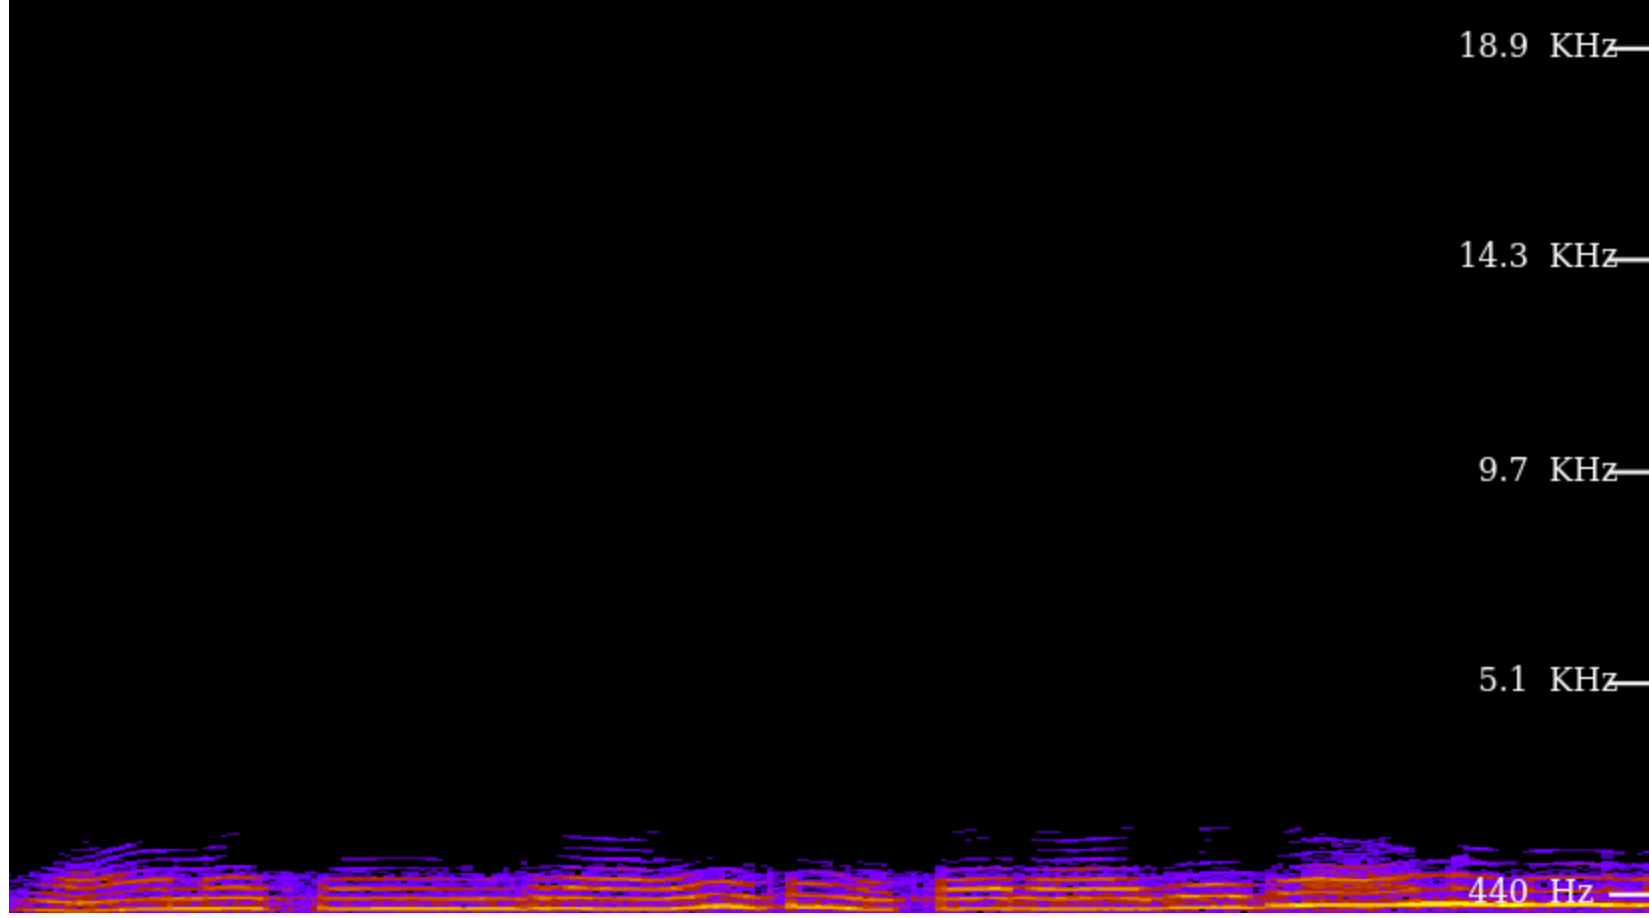
\includegraphics[width=0.8\columnwidth]{figs/afterfiltering.png}
    \caption{Spectrogram of the audio file after Filtering}
    \label{fig:afterfiltering}
\end{figure}
\end{enumerate}

\section{DIFFERENCE EQUATION}
\begin{enumerate}[label=\thesection\arabic*.,ref=\thesection.\theenumi]
\item Let
\begin{align}
x(n) &= \cbrak{\underset{\uparrow}{1},2,3,4,2,1}
\end{align}
Sketch $x(n)$.
\item Let 
\begin{align}
y(n) +\frac{1}{2}y(n-1) &= x(n) + x(n-2), \label{2.2}\nonumber \\
& \hspace{2cm} y(n)=0, n<0
\end{align}
\end{enumerate}
\solution  C code for generating values of y(n):
\begin{lstlisting}
https://github.com/BATCHUISHITHA/EE-1205/blob/main/audio_filtering/codes/2.2.c
\end{lstlisting} 
Python code for plotting x(n) and y(n):
\begin{lstlisting}
https://github.com/BATCHUISHITHA/EE-1205/blob/main/audio_filtering/codes/2.2.py
\end{lstlisting}
\begin{figure}[ht]
	\centering
	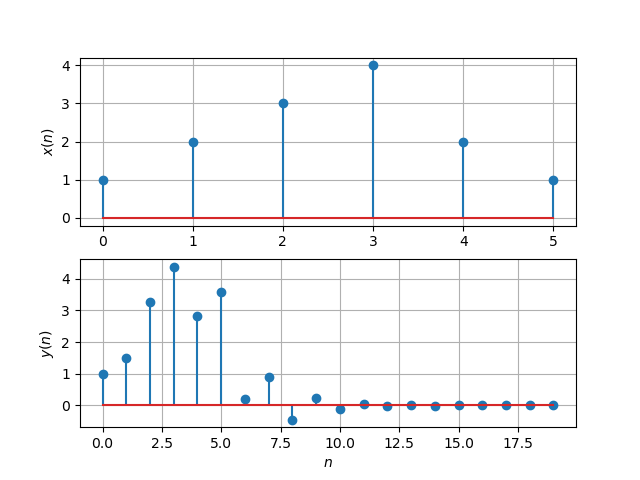
\includegraphics[width=\columnwidth]{figs/2.2.png}
	\caption{Plot of $x(n)$ and $y(n)$}
	\label{fig:2.2}
\end{figure}

\section{Z-Transform}

\begin{enumerate}[label=\thesection.\arabic*]
\item The $Z$-transform of $x(n)$ is defined as
\begin{equation}
X(z)=\systemZ{}\cbrak{x(n)}=\sum _{n=-\infty }^{\infty }x(n)z^{-n} \label{z-transform}
\end{equation}
Show that
\begin{equation}
\systemZ{} \cbrak{x(n-1)} = z^{-1}X(z) \label{z1}
\end{equation}
and find
\begin{equation}
	\systemZ{} \cbrak{x(n-k)}. 
\end{equation}
\solution 
Let
\begin{align}
y(n) &= x(n-k) \label{eq:l1}
\end{align}
Taking z-transform
\begin{align}
\mathcal{Z}\brak{y(n)} &= \mathcal{Z}\brak{x(n-k)} \label{eq:l2}
\end{align}
Simplifying LHS
\begin{align}
Y(z) &= \sum_{n=-\infty}^{\infty} y(n)z^{-n} 
\end{align}
From \eqref{eq:l1}
\begin{align}
Y(z) &= \sum_{n=-\infty}^{\infty} x(n-k) z^{-n} \label{eq:l3}
\end{align}
Let 
\begin{align}
n-k &= s  \\\implies
n &= s+k \label{eq:l4}
\end{align}
From \eqref{eq:l3} and \eqref{eq:l4}
\begin{align}
Y(z) &= \sum_{s=-\infty}^{\infty} x(s) z^{-(s+k)} \\
&= z^{-k}\sum_{s=-\infty}^{\infty} x(s) z^{-s} 
\end{align}
As variable in Z-transform is dummy, on replacing it, we get
\begin{align}
Y(z) &= z^{-k}\sum_{n=-\infty}^{\infty} x(n) z^{-n} \\
&= z^{-k}X(z) \label{eq:l5}
\end{align}
From \eqref{eq:l2} and \eqref{eq:l5}
\begin{align}
\mathcal{Z}\brak{x(n-k)} &= z^{-k}X(z) \label{z2}
\end{align}
Put $k = 1$ resulting in \eqref{z1} \\
Hence proved \\
\item Find
\begin{align}
H(z)=\frac{Y(z)}{X(z)}
\end{align}
from \eqref{2.2} assuming that the Z-transform is a linear operation.\\
\solution Applying Z-transform on both sides of \eqref{2.2}
\begin{align}
Y(z)+\frac{1}{2}z^{-1}Y(z) &= X(z)+z^{-2}X(z) \\
\implies H(z)= \frac{Y(z)}{X(z)}&=\frac{1+z^{-2}}{1+\frac{1}{2}z^{-1}} \label{3.2}
\end{align}
\item Find the Z transform of 
\begin{equation}
\delta(n)
=
\begin{cases}
1 & n = 0
\\
0 & \text{otherwise}
\end{cases}
\end{equation}
and show that the $Z$-transform of
\begin{equation}
\label{u(n)}
u(n)
=
\begin{cases}
1 & n \ge 0
\\
0 & \text{otherwise}
\end{cases}
\end{equation}
is
\begin{equation}
U(z) = \frac{1}{1-z^{-1}}, \quad \abs{z} > 1
\end{equation}
\solution
 \begin{align}
    Z\{ \delta[n] \} &= \sum_{n=-\infty}^{\infty} \delta[n] \cdot z^{-n} \\
                     &= z^0 \\
                     &= 1
\end{align}
and from \eqref{u(n)},
\begin{align}
U(z) &= \sum _{n= 0}^{\infty}z^{-n} \\
&=\frac{1}{1-z^{-1}}, \quad \abs{z} > 1
\end{align}
using the formula for the sum of an infinite geometric progression.
\item Show that 
\begin{equation}
\label{eq:anun}
a^nu(n) \xleftrightarrow{\systemZ{}}\frac{1}{1-az^{-1}} \quad \abs{z} > \abs{a}
\end{equation}
\solution 
\begin{align}
	\systemZ{}\cbrak{a^nu(n)}&= \sum_{n = 0}^{\infty}\brak{az^{-1}}^n \\
			&= \frac{1}{1-az^{-1}} \quad \abs{z} > \abs{a} \label{3.4}
\end{align}
\item Let
\begin{align}
H(e^{j\omega})&=H(z=e^{j\omega}).
\end{align}
Plot $\abs{H(e^{j\omega})}$.Comment.$\abs{H(e^{j\omega})}$ is known as \textit{Discrete Time Fourier Transform} (DTFT) of x(n).\\
\solution
Substituting $z=e^{j\omega}$ in \eqref{3.2},
\begin{align}
H(e^{j\omega})&=\frac{1+e^{-2j\omega}}{1+\frac{1}{2}e^{-j\omega}} \\
\abs{H(e^{j\omega})} &= \abs{\frac{1+\cos2\omega -j\sin 2\omega }{1+\frac{1}{2}\brak{\cos\omega-j\sin\omega}}} \\
&= \sqrt{\frac{\brak{1+\cos2\omega}^2+\brak{\sin 2\omega}^2}{\brak{1+\frac{1}{2}\cos\omega}^2+\brak{\frac{1}{2}\sin\omega}^2}}\\
&= \frac{4\abs{\cos\omega}}{\sqrt{5+4\cos\omega}}\\
\abs{H(e^{j(\omega+2\pi)})}&=\abs{\frac{1+e^{-2j(\omega+2\pi)}}{1+\frac{1}{2}e^{-j(\omega+2\pi)}}} \\
&= \frac{4\abs{\cos\omega}}{\sqrt{5+4\cos\omega}} \\
&= \abs{H(e^{j\omega})} 
\end{align}
Therefore, the fundamental period of $H(e^{j\omega})$ is $2\pi$.\\
$\implies$ DTFT of a signal is always periodic.\\ 
The following code plots \eqref{fig:dtft}:
\begin{lstlisting}
https://github.com/BATCHUISHITHA/EE-1205/blob/main/audio_filtering/codes/3.5.py
\end{lstlisting}
\begin{figure}[ht]
	\centering
	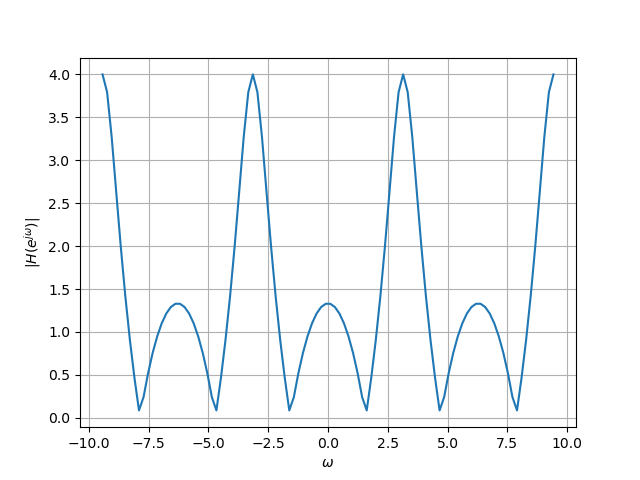
\includegraphics[width=\columnwidth]{figs/3.4.png}
	\caption{$\abs{H\brak{e^{j\omega}}}$}
	\label{fig:dtft}
\end{figure}
\end{enumerate}

\section{Impulse Response}
\begin{enumerate}[label=\thesection.\arabic*]
\item \label{prob:impulse_resp}
Find an expression for $h(n)$ using $H(z)$, given that 
\begin{equation}
h(n) \xleftrightarrow{\systemZ{}} H(z)  \label{4.1}
\end{equation}
and there is a one to one relationship between $h(n)$ and $H(z)$. $h(n)$ is known as the {\em impulse response} of the
system defined by \eqref{2.2}.\\
\solution From \eqref{3.2},
\begin{align}
H(z) &= \frac{1}{1 + \frac{1}{2}z^{-1}} + \frac{ z^{-2}}{1 + \frac{1}{2}z^{-1}}
\\
\implies h(n) &= \brak{-\frac{1}{2}}^{n}u(n) + \brak{-\frac{1}{2}}^{n-2}u(n-2)
\end{align}
from \eqref{3.4} and \eqref{z2}.
\item Sketch $h(n)$. Is it bounded?Convergent?\\
\solution
Yes, h(n) is convergent and bounded.\\
The following code plots h(n) vs n.
\begin{lstlisting}
https://github.com/BATCHUISHITHA/EE-1205/blob/main/audio_filtering/codes/4.2.py
\end{lstlisting}
\begin{figure}[ht]
	\centering
	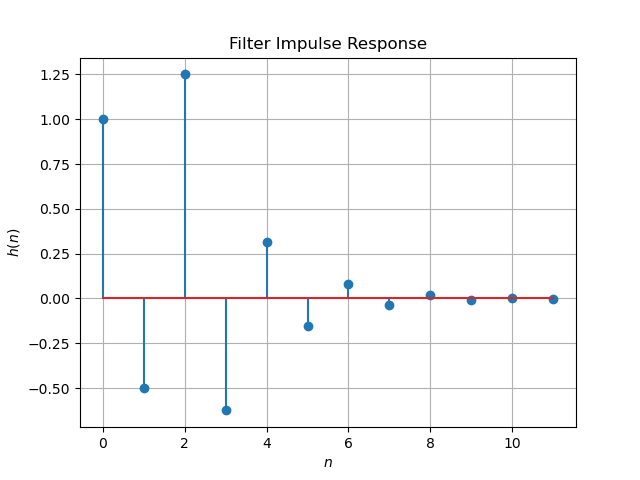
\includegraphics[width=\columnwidth]{figs/4.2.png}
	\caption{$h(n)$ as the inverse of $H(z)$}
	\label{fig:4.2}
\end{figure}
\item The system with h(n) is defined to be stable if
\begin{align}
\sum_{n=-\infty}^{\infty}h(n) < \infty \label{hn}
\end{align}
Is the system defined by \eqref{2.2} stable for impulse response in \eqref{4.1}?\\
\solution For stable system \eqref{hn} must be converging.\\
For n $\rightarrow$ $\infty$,
\begin{align}
u(n)=u(n-2)=1\\
\implies h(n) &= \brak{-\frac{1}{2}}^{n}+ \brak{-\frac{1}{2}}^{n-2}
\end{align}
Since, both terms of h(n) tends to 0 as n$\rightarrow$ $\infty$, h(n)$\rightarrow$ $0$.\\
$\implies$ output remains bounded for bounded inputs,ie: $h(n)$ is stable.
\item Compute  and sketch h(n) using 
\begin{align}
h(n) + \frac{1}{2}h(n-1) &= \delta(n)+\delta(n-2)
\end{align}
This is the definition of h(n).\\
\solution The following code plots \eqref{fig:4.4} .\\
Note that this is same as \eqref{fig:4.2}.
\begin{lstlisting}
https://github.com/BATCHUISHITHA/EE-1205/blob/main/audio_filtering/codes/4.4.py
\end{lstlisting}
\begin{figure}[ht]
	\centering
	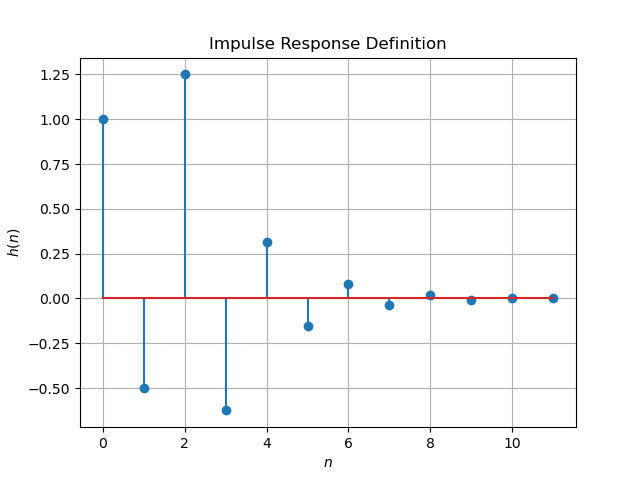
\includegraphics[width=\columnwidth]{figs/4.4.png}
	\caption{$h(n)$ from the definition}
	\label{fig:4.4}
\end{figure}
\item Compute 
\begin{equation}
\label{eq:convolution}
y(n) = x(n)*h(n) = \sum_{k=-\infty}^{\infty}x(k)h(n-k)
\end{equation}
Comment. The operation in \eqref{eq:convolution} is known as
{\em convolution}.\\
\solution The following code plots Fig. \ref{fig:4.5}. \\
Note that this is the same as $y(n)$ in  Fig:\ref{fig:2.2}. 

\begin{lstlisting}
https://github.com/BATCHUISHITHA/EE-1205/blob/main/audio_filtering/codes/4.5.py
\end{lstlisting}
\begin{figure}[ht]
\centering
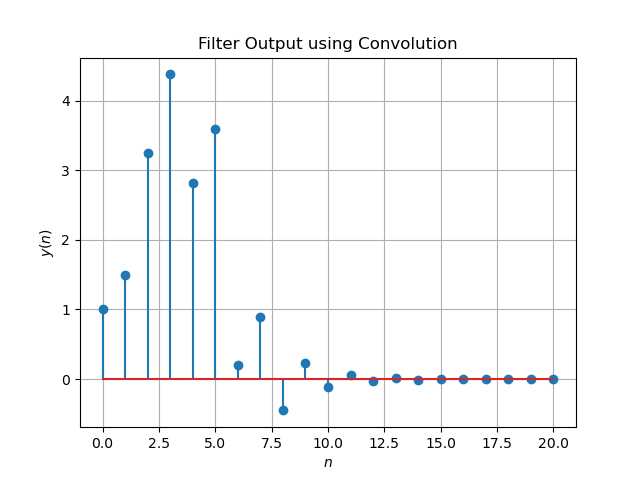
\includegraphics[width=\columnwidth]{figs/4.5.png}
\caption{$y(n)$ from the definition of convolution}
\label{fig:4.5}
\end{figure}
\newpage
\item Show that
\begin{equation}
y(n) =  \sum_{k=-\infty}^{\infty}x(n-k)h(k)
\end{equation}
\solution
In \eqref{eq:convolution}, replacing $k$ by $n - k$ 
\begin{align}
y\brak{n} &= \sum_{n-k=-\infty}^{\infty}x(n-k)h(n-(n-k)) \\
 &= \sum_{k=-\infty}^{\infty}x(n - k)h(k)
\end{align}
\end{enumerate}

\section{DFT AND FFT}
\begin{enumerate}[label=\thesection.\arabic*]
\item Compute
\begin{equation}
X(k) \define \sum _{n=0}^{N-1}x(n) e^{\frac{-2\pi jkn}{N}}, \quad k = 0,1,\dots, N-1
\end{equation}
and $H(k)$ using $h(n)$.
\item Compute 
\begin{align}
Y(k) = X(k)H(k) \label{eq:5.2.1}
\end{align}
\item Compute
\begin{align}
y\brak{n}={\frac {1}{N}}\sum _{k=0}^{N-1}Y\brak{k}\cdot e^{\frac{-2\pi jkn}{N}} ,\quad n = 0,1,\dots, N-1\label{eq:5.3.1}
\end{align}
\solution The above three questions are solved using the code below.\\
\begin{lstlisting}
https://github.com/BATCHUISHITHA/EE-1205/blob/main/audio_filtering/codes/5.py
\end{lstlisting}
\begin{figure}[ht]
	\centering
	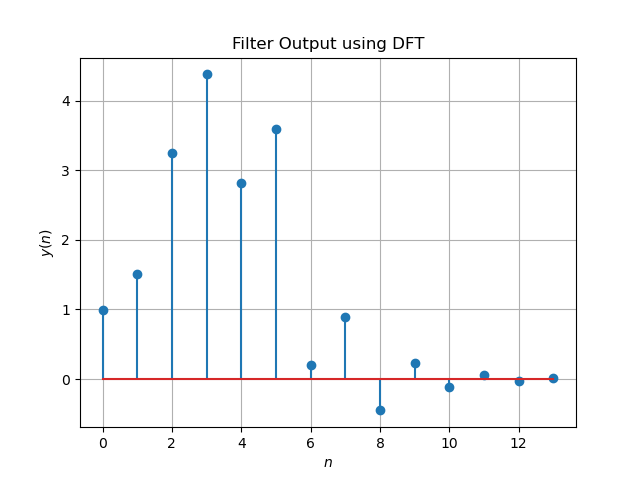
\includegraphics[width=\columnwidth]{figs/5.png}
	\caption{$y(n)$ from the DFT}
	\label{fig:5}
\end{figure}
\item Repeat the previous exercise by computing $X(k), H(k)$ and $y(n)$ through FFT and IFFT.\\
\solution This code verifies the result by plotting the result obtained from DFT,IDFT and the result obtained from FFT,IFFT.
\begin{lstlisting}
https://github.com/BATCHUISHITHA/EE-1205/blob/main/audio_filtering/codes/5.4.py
\end{lstlisting}
\begin{figure}[ht]
	\centering
	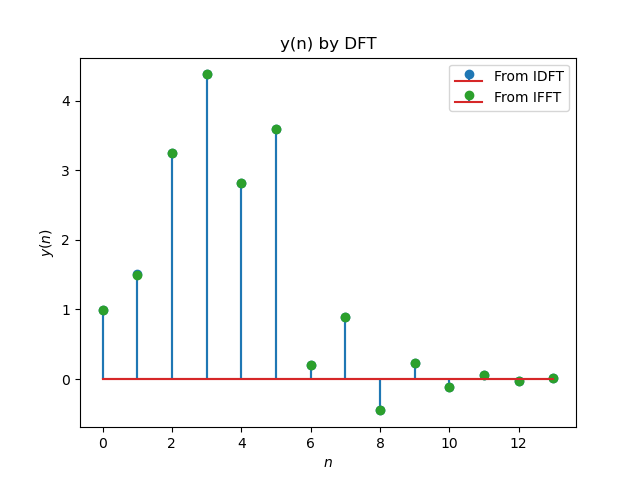
\includegraphics[width=\columnwidth]{figs/5.4.png}
	\caption{$y(n)$ from the DFT, IDFT and from the FFT,IFFT are plotted and verified}
	\label{fig:5.4}
\end{figure}
\item Wherever possible, express all the above equations as matrix equations.\\
\solution The DFT matrix is defined as : 
\begin{align}
	\mtx{W} = 
	\begin{pmatrix}
		\omega^0 & \omega^0 & \ldots & \omega^0 \\
		\omega^0 & \omega^1 & \ldots & \omega^{N - 1} \\
		\vdots & \vdots & \ddots & \vdots \\
		\omega^0 & \omega^{N - 1} & \ldots & \omega^{(N -1)(N - 1)}
	\end{pmatrix}
\end{align}
where $\omega=e^{-\frac{j2\pi}{N}}$ . Now any DFT equation can be written as
\begin{align}
    \mtx{X} = \mtx{W}\mtx{x}
\end{align}
\noindent where  $\mtx{x}$ is the original signal and $\mtx{X}$ is the frequency-domain representation. 
\begin{align}
	\mtx{x} = 
	\begin{pmatrix}
		x(0) \\ x(1) \\ \vdots \\ x(n - 1)
	\end{pmatrix}
\end{align}
\begin{align}
	\mtx{X} = 
	\begin{pmatrix}
		X(0) \\ X(1) \\ \vdots \\ X(n - 1)
	\end{pmatrix}
\end{align}
Thus we can rewrite  \eqref{eq:5.2.1} as:
\begin{align}
	\mtx{Y} = \mtx{X}\odot\mtx{H} = \brak{\mtx{W}\mtx{x}}\odot\brak{\mtx{W}\mtx{h}}
\end{align}
where the $\odot$ represents the Hadamard product which performs element-wise multiplication.
This is specifically called "SCHUR PRODUCT" when defined for matrices.
\begin{lstlisting}
https://github.com/BATCHUISHITHA/EE-1205/blob/main/audio_filtering/codes/5.5.py
\end{lstlisting}
\begin{figure}[ht]
	\centering
	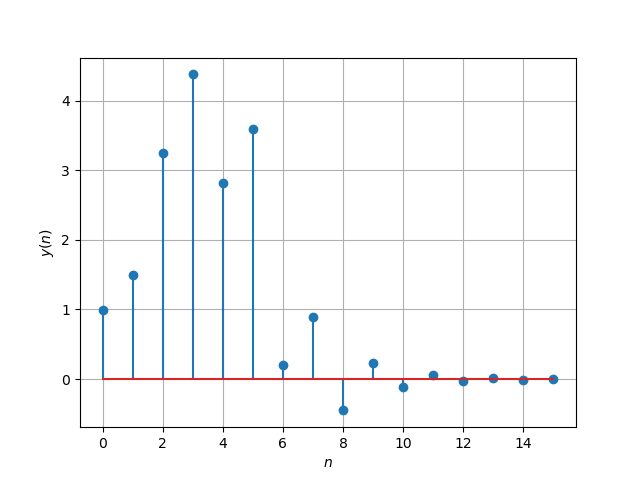
\includegraphics[width=\columnwidth]{figs/5.5.png}
	\caption{$y(n)$ obtained from DFT matrix }
	\label{fig:5.5}
\end{figure}
\end{enumerate}

\section{EXERCISES}
Answer the following questions by looking at the python code in Problem:\eqref{1.2}
\begin{enumerate}[label=\thesection.\arabic*]
\item The command
\begin{lstlisting}
output_signal = signal.lfilter(b, a, input_signal)
\end{lstlisting}
in Problem:\eqref{1.2}  is executed through the following difference equation
\begin{equation}
 \sum _{m=0}^{M}a\brak{m}y\brak{n-m}=\sum _{k=0}^{N}b\brak{k}x\brak{n-k} \label{6.1}
\end{equation}
where the input signal is $x(n)$ and the output signal is $y(n)$ with initial values all 0. Replace
\textbf{signal.filtfilt} with your own routine and verify.\\
\solution The below is the code for output of an audio signal with and without using inbuilt function signal.lfilter\\
\begin{lstlisting}
https://github.com/BATCHUISHITHA/EE-1205/blob/main/audio_filtering/codes/6.1.py
\end{lstlisting}
\begin{figure}[ht]
	\centering
	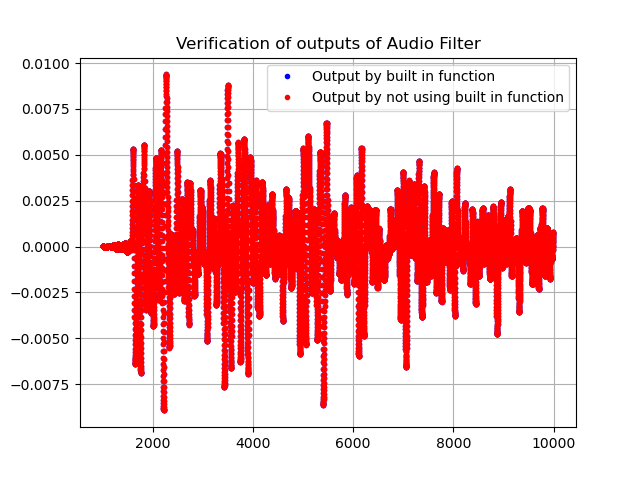
\includegraphics[width=\columnwidth]{figs/6.1.png}
	\caption{output of an audio signal with and without inbuilt function signal.lfilter are plotted and verified}
	\label{fig:6.1}
\end{figure}
\item Repeat all the exercises in the previous sections for the above $a$ and $b$.\\
\solution The code in \ref{1.2} generates the values of $a$ and $b$  which can be used to generate a difference equation.\\
And,
\begin{align}
    M &= 5\\
    N&=5
\end{align}
From \ref{6.1} 
\begin{align}
    &a\brak{0}y\brak{n} + a\brak{1}y\brak{n-1}+a\brak{2}y\brak{n-2}+a\brak{3}\\ \notag &y\brak{n-3} + a\brak{4}y\brak{n-4} =   b\brak{0}x\brak{n} + b\brak{1}x\brak{n-1}\\ \notag &+b\brak{2}x\brak{n-2}+b\brak{3}x\brak{n-3} + b\brak{4}x\brak{n-4} 
\end{align}
Difference Equation is given by :
\begin{align}
	&y(n) - \brak{3.63}y(n - 1) + \brak{4.95}y(n - 2) \nonumber \\
	&- \brak{3.01}y(n - 3) + \brak{0.69}y(n - 4) \nonumber \\
	&= \brak{2.15\times 10^{-5}}x(n) + \brak{8.60 \times 10^{-5}}x(n - 1) \nonumber \\
	&+ \brak{1.29 \times 10^{-4}}x(n - 2) + \brak{8.60 \times 10^{-5}}x(n - 3) \nonumber \\
	&+ \brak{2.15\times 10^{-5}}x(n - 4)
\end{align}
From \eqref{6.1} 
\begin{align}
    H(z) &= \frac{b_0 + b_1 z^{-1} + b_2 z^{-2} + \ldots + b_M z^{-N}}{a_0 + a_1 z^{-1} + a_2 z^{-2} + \ldots + a_N z^{-M}}\\
    H(z) &= \frac{\sum_{k = 0}^{N}b(k)z^{-k}}{\sum_{k = 0}^{M}a(k)z^{-k}} \label{eq:6.2}
\end{align}
Partial fraction on \eqref{eq:6.2} can be generalised as:
\begin{align}
    H\brak{z}&= \sum_{i}\frac{r(i)}{1 - p(i)z^{-1}} + \sum_{j}k(j)z^{-j}
	\label{eq:6.2.1}
\end{align}
Now,
\begin{align}
    a^{n}u\brak{n} \xleftrightarrow{\systemZ{}}  \frac{1}{1-az^{-1}} \label{eq:6.2.2}\\
    \delta\brak{n-k} \xleftrightarrow{\systemZ{}} z^{-k}\label{eq:6.2.3}
\end{align}
Taking inverse z transform of \eqref{eq:6.2.1} by using \eqref{eq:6.2.2} and \eqref{eq:6.2.3}
\begin{align}
h(n) &= \sum_{i}r(i)[p(i)]^nu(n) + \sum_{j}k(j)\delta(n - j)
	\label{eq:6.2.4}
\end{align}
The below code computes the values of $r\brak{i},p\brak{i} , k\brak{i}$ and plots $h\brak{n}$
\begin{lstlisting}
https://github.com/BATCHUISHITHA/EE-1205/blob/main/audio_filtering/codes/6.2.py
\end{lstlisting}
\begin{table}[H]
    \centering
    \renewcommand\thetable{1}
    \setlength{\extrarowheight}{9pt}
    \resizebox{0.51\textwidth}{!}{
    \begin{tabular}{|c|c|c|}
    \hline
    \textbf{$r\brak{i}$} & \textbf{$p\brak{i}$} & \textbf{$k\brak{i}$} \\ \hline
    $0.58129538 -2.51766121j$ &0.13676769 +0.19533079j&$2.02482078$  \\ \hline
    $0.58129538 +2.51766121j$ &0.13676769 -0.19533079j&$-$  \\ \hline
    $-0.40482158+0.3262658j$ &0.188968140+0.6515556j&$-$  \\ \hline
    $-0.40462158-0.3262658j$ &0.188968140-0.6515556j&$-$  \\ \hline
    \end{tabular}}
    \caption{Values of $ r(i) , p(i) , k(i)$}
    \label{tab:values of r(i) , p(i) , k(i)}
    \end{table}

\begin{figure}[ht]
\centering
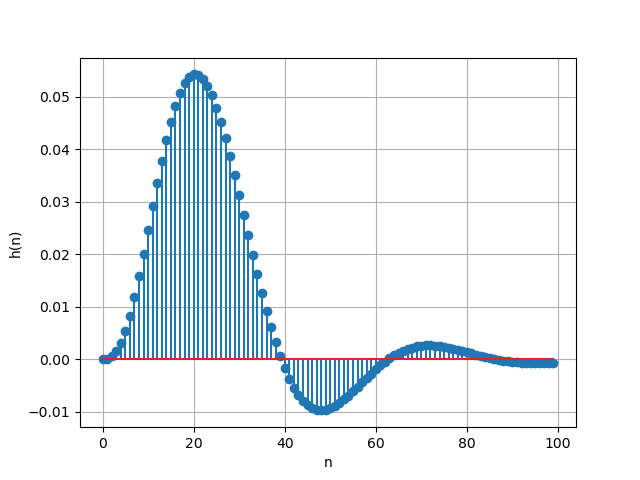
\includegraphics[width=1\columnwidth]{figs/6.2.png}
\caption{h(n) of Audio Filter}
\label{fig:6.2}
\end{figure}
\textbf{Stability of h(n)}:\\
According to \eqref{hn}
\begin{align}
H\brak{z} &= \sum_{n = 0}^{\infty} h\brak{n}z^{-n}\\
H(1)&= \sum_{n = 0}^{\infty}h(n)  = \frac{\sum_{k = 0}^{N}b(k)}{\sum_{k = 0}^{M}a(k)}< \infty
\end{align}
As both $a\brak{k}$ and $b\brak{k}$ are finite length sequences they converge.\\
The below code plots Filter frequency response
\begin{lstlisting}
https://github.com/BATCHUISHITHA/EE-1205/blob/main/audio_filtering/codes/6.2.1.py
\end{lstlisting}
\begin{figure}[ht]
\centering
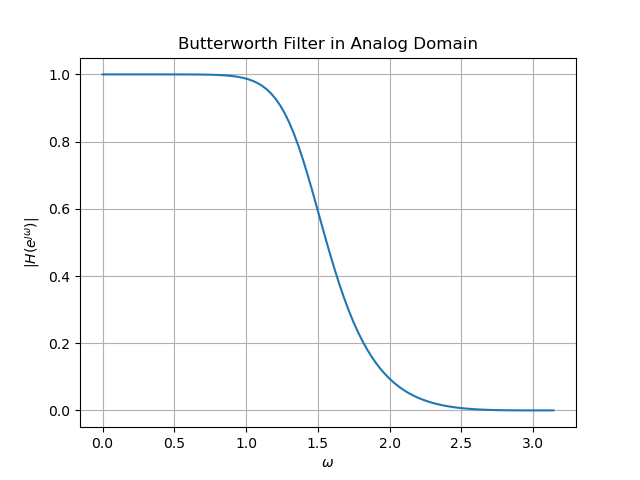
\includegraphics[width=1\columnwidth]{figs/6.2.1.png}
\caption{Frequency Response of Audio Filter}
\label{fig:6.2.1}
\end{figure}
The below code plots the Butterworth Filter in analog domain by using bilinear transform.
\begin{align}
    z=\frac{1+sT/2}{1-sT/2}
\end{align}
\begin{lstlisting}
https://github.com/BATCHUISHITHA/EE-1205/blob/main/audio_filtering/codes/6.2.2.py
\end{lstlisting}
\begin{figure}[H]
\centering
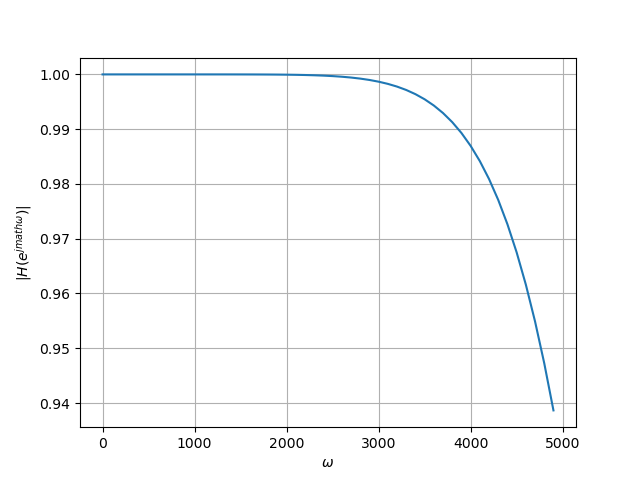
\includegraphics[width=1\columnwidth]{figs/6.2.2.png}
\caption{Butterworth Filter Frequency response in analog domain}
\label{fig:6.2.2}
\end{figure}
The below code plots the Pole-Zero Plot of the frequency response.
\begin{lstlisting}
https://github.com/BATCHUISHITHA/EE-1205/blob/main/audio_filtering/codes/6.2.3.py
\end{lstlisting}
\begin{figure}[H]
\centering
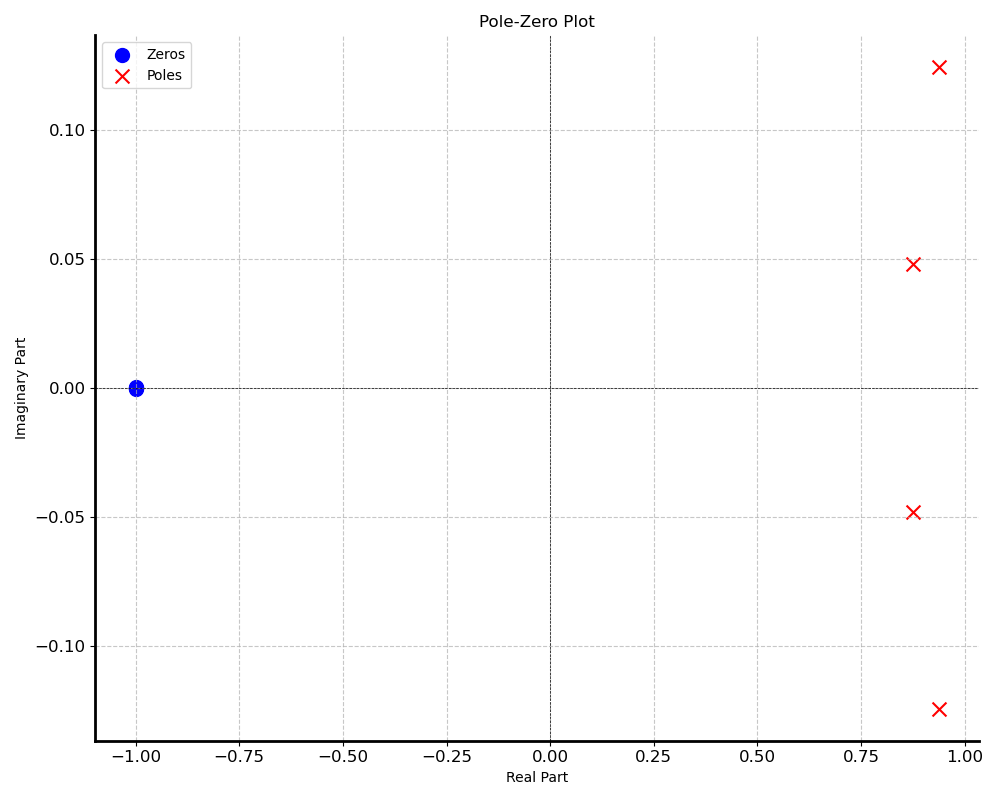
\includegraphics[width=1\columnwidth]{figs/6.2.3.png}
\caption{There are complex poles. So $h\brak{n}$ should be damped sinusoid.}
\label{fig:6.2.3}
\end{figure}

\item What is the sampling frequency of the input signal? \\
\solution The sampling frequency of the input signal is 44.1kHz.
\item What is type, order and  cutoff-frequency of the above butterworth filter\\
\solution The given butterworth filter is lowpass with order=$4$ and cutoff-frequency=$1kHz$.
\item Modifying the code with different input parameters and to get the best possible output.\\
\solution A better filtering was found on setting the order of the filter to be 5.
\end{enumerate}
\end{document}
